\section{Modelo Inicial}

Algo que introduzca esto

\vspace{3mm}

Dado un grafo $G = (V,E\cup A)$, $R \subseteq E\cup A$ como el conjunto de ejes obligatorios de recorrer,  
$t:E\cup A\rightarrow \mathbb{R}$ como el tiempo en recorrer el eje $ij$, $q:E\cup A\rightarrow \mathbb{R}$ 
como la demanda del eje $ij$ y $W$ la capacidad de cada camión, definimos las siguientes variables.

\begin{align*}
    X^p_{ij} &= 
    \begin{cases}
        1 & \text{si el eje } ij \text{ fue satisfecho en el viaje } p \\
        0 & \text{caso contrario}
    \end{cases} \\
    Y^p_{ij} &= \text{Cantidad de veces que el eje } ij \text{ fue recorrido sin recoger en el viaje } p \\
    F^p_{ij} &= \text{Flujo del eje } ij \text{ en el viaje } p \\
\end{align*}

El modelo que en una primera instancia resuelve el problema es el siguiente. Como notación vamos a usar $t_{ij}$ 
en lugar de $t(ij)$ para referirnos al tiempo en recorrer el eje $ij$, además usaremos $S = E\cup A$.

\begin{align}
    \min \quad & \sum^P_{p=1}(\sum_{ij\in R}t_{ij}X^p_{ij} + \sum_{ij\in S}t_{ij}Y^p_{ij}) \\
    \text{sujeto a} \quad & \sum_{j/ij\in S} Y^p_{ij} + \sum_{j/ji\in R} X^p_{ij} = \sum_{j/ji\in S} Y^p_{ji} + \sum_{j/ij\in R} X^p_{ji} & \forall i \text{ } \forall p \\
    & \sum_{p=1} X_{ij}^p = 1 & \forall ij \in R \cap A \\
    & \sum_{p=1} (X_{ij}^p + X_{ji}^p) = 1 & \forall ij \in R \cap E \\
    & \sum_{j:(0j)\in S} Y^p_{0j} + \sum_{j:(0j)\in R} X^p_{0j} \leq 1 & \forall p \\
    & \sum_{j:(ji)\in S} F^p_{ji} - \sum_{j:(ij)\in R} F^p_{ij} = \sum_{j:(ji)\in R}q_{ij} X_{ji}^P & \forall i \text{ } \forall p \\
    & \sum_{j:(0j) \in S} F^p_{0j} = \sum_{(ij)\in R} q_{ij}X_{ij}^p & \forall i \forall p \\
    & \sum_{i:(i0) \in S} F^p_{i0} = \sum_{i:(i0)\in R} q_{i0}X_{i0}^p & \forall p \\
    & F^p_{ij} \leq W(y^p_{ij} + x^p_{ij}) & \forall(i,j) \in S, \forall p \\
    & X^p_{ij} \in \{0,1\} & \forall(i,j) \in R, \forall p \\
    & F^p_{ij} \geq 0 & \forall(i,j) \in S, \forall p \\
    & Y^p_{ij} \geq 0 \text{ entera} & \forall(i,j) \in S, \forall p
\end{align}

La función objetivo (1) del problema representa el costo total del recorrido, es decir, el costo 
de recoger residuos y el de recorrer por ejes sin recoger. La condición (2) impone continuidad al 
recorrido sobre cada nodo, que todo nodo tenga la misma cantidad de entradas que salidas. 
Luego, (3) y (4), obligan a recorrer todos los arcos y aristas respectivamente. 
En la restricción (5) nos aseguramos de que en cada camión salga del depósito a lo sumo una vez. 
Luego, las condiciones (6)-(9) tienen la función de conservar el flujo y forzar la conectividad entre cada nodo. 
Por otro lado, la condición (9) impone una cota súperior que garantiza que la capacidad $W$ no se súpere. 
Vale aclarar que este modelo, no tiene en consideración al depósito como nodo intermedio.

[Siento que quedó medio vacío]

\section{Evitando movimientos prohibidos}

El modelo inicial resuelve el problema, satisfaciendo tanto la conectividad como la demanda. 
Sin embargo, no tiene en cuenta ciertas reglas de tránsito que nosotros debemos respetar. 
Estas reglas son: los \textbf{giros en U} y los \textbf{giros a la izquierda prohibidos}.

\vspace{3mm}


Para resolver ambos problemas debemos contener más información en nuestras intersecciones para poder manejar 
cada caso. Para ello, vamos a \textbf{expandir} cada intersección convirtiendo nuestro grafo en un 
\textit{súper-grafo}.  

\subsection{Súper-Grafo}

Dado el grafo $G = (V, E \cup A)$ nuestro súper-grafo $SG$ representará cada nodo con un \textit{súper-nodo} 
y cada arista con una \textit{súper-arista}. El súper-grafo es un grafo dirigido que expande un grafo $G$, 
es decir, tantos los nodos como las aristas en el grafo se convierten en conjuntos de nodos y aristas 
respectivamente. 

\vspace{3mm}

Definamos nuestro súper-grafo $SG = (SV,SE)$, para cada vértice $v \in V$ vamos a representarlo como 
el conjunto de nodos tal que $uv \in E\cup A$. Es decir, cada nodo $uv \in SV$, indica que nos encontramos 
en la intersección $v$ viniendo desde la intersección $u$. 
Por otro lado, para cada par vértices $uv,vw \in SV$ existe un arco $((uv),(vw))$ si y sólo si existe 
el camino $uvw$ en $G$. Formalmente:

\begin{itemize}
    \item $SV = E \cup A$
    \item $SA = \{((uv),(kw)) : (uv),(kw) \in SV \land v = k \land u \neq w \} $
\end{itemize}

\begin{figure}[h]
\centering

\begin{subfigure}{0.2\linewidth}
\centering
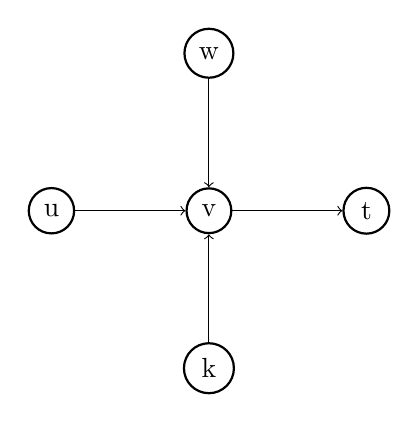
\begin{tikzpicture}
  \begin{scope}[every node/.style={circle, thick, draw}]
    \node (u) at (-2,0) {u};
    \node (w) at (0,2) {w};
    \node (t) at (2,0) {t};
    \node (k) at (0,-2) {k};
    \node (v) at (0,0) {v};
  \end{scope}
  \draw[->] (u) -- (v);
  \draw[->] (v) -- (t);
  \draw[->] (w) -- (v);
  \draw[->] (k) -- (v);
\end{tikzpicture}
\caption{Grafo}
\label{fig:grafo}
\end{subfigure}
\hfill
\begin{subfigure}{0.45\linewidth}
\centering
\begin{tikzpicture}[scale=0.9, transform shape]
  \begin{scope}[every node/.style={circle, thick, draw}]
    \node (uv) at (-4,0)  {$uv$};
    \node (vu) at (-4,-1.7) {$vu$};

    \node (vw) at (-1,1.6) {$vw$};
    \node (wv) at (1.2,1.6) {$wv$};

    \node (vt) at (4,0) {$vt$};
    \node (tv) at (4,-1.7) {$tv$};

    \node (vk) at (-1,-3) {$vk$};
    \node (kv) at (1.2,-3) {$kv$};
  \end{scope}

  \draw[-{Stealth}] (uv) -- (vw);
  \draw[-{Stealth}] (uv) -- (vt);
  \draw[-{Stealth}] (uv) -- (vk);

  \draw[-{Stealth}] (wv) -- (vu);
  \draw[-{Stealth}] (wv) -- (vt);
  \draw[-{Stealth}] (wv) -- (vk);

  \draw[-{Stealth}] (tv) -- (vu);
  \draw[-{Stealth}] (tv) -- (vw);
  \draw[-{Stealth}] (tv) -- (vk);

  \draw[-{Stealth}] (kv) -- (vu);
  \draw[-{Stealth}] (kv) -- (vw);
  \draw[-{Stealth}] (kv) -- (vt);
\end{tikzpicture}
\caption{Supergrafo}
\label{fig:supergrafo}
\end{subfigure}
\label{fig:ambos}
\end{figure}

Dado el nuevo modelo con el súper-grafo, podemos fácilmente prohibir los giros en U, ya que no 
tenemos forma de realizarlo. Luego, para prohibir los giros a la izquierda basta con eliminar todas 
las aristas tal que representen tal giro y no tengan un semáforo con giro habilitado.

\newpage

\section{Fix \& Optimize}

Esta heurística nace de la motiviación de querer mejorar los tiempos del modelo inical, ya que este 
puede demandar demasiado tiempo al buscar optimalidad ya que en el espacio de búsqueda es consideradamente
grande. Por otro lado, con Fix \& Optimize se reduce temporalmente este espacio, obteniendo solcuiones locales
con mayor velocidad. Para lograr tal velocidad se debe comenzar con una solcuión facitble del MIP inicial,
para luego fijar variables y optimizar las libres. 

\vspace{3mm}

Es una heurística
iterativa donde, mientras haya una mejora, se elige un vecindario, se fijan las variables de recorrido con 
el valor de la solcuión incumbente salvo las de la zona elegida y se resuelve. Finaliza cuando se llega 
a un límite de iteraciones sin mejora. El algoritmo  itera hasta agotar la cantidad de iteraciones que 
tiene disponible o si durante 20 iteraciones no mejora.

Lo interesante de esta técnica es como elegir ese vecindario. En esta tesis vamos a analizar 3
maneras de elegir: Aleatorio, Máxima costo de recorridos sin servicio y K-máximas costo de recorridos sin servicio.

\subsection{Selección de vecindarios}

\textbf{Aleatoria}: La selección aleatoria elige una arista unifromemente y selecciona todas las aristas
a distancia $d$.

\textbf{Máxima costo de recorridos sin servicio}: Para este caso se elige la arista con mayor costo de recorridos 
sin servicio ya que será las que más combinaciones acepte y por ende la que tenga más chances de ser modificada.
Para calcular el costo de recorrido sin servicio multiplicamos la cantidad de pasadas sin realizar servicio por
el tiempo que toma recorrer dicha arista.

\textbf{K-máxima costo de recorridos sin servicio}: Esta selección realiza un top-$k$ con los parámetros $k$, $d$ y 
la tolerancia en el gap. La idea es que si se encuentra una mejora entonces reducimos el $k$, la cantidad de
vecindarios de exploración, la $d$, el tamaño de los vecindario y mantenemos una tolerancia en el gap
más relajada. Sin embargo, si no mejora, alterna entre iteraciones la incrementación de $k$ o $d$. Si durante
5 iteraciones no se encontró una solución mejor se reduce la tolerancia en el gap.

\section{Zonificación}

A pesar de que el municipio nos dio zonas establecidas siguiendo los barrios, nosotros elegimos zonificar cada una de estas grandes zonas. El motivo de esta zonificación se debe a que el modelo anterior teniendo $P$ camiones tiene muchas posibilidades y es difícil hacer que respete una condición que exige el municipio que es que los camiones se crucen lo menos posible en cuanto a rutas. Por lo tanto, en lugar de resolver el problema con $P$ camiones podemos resolver sub-zonas por separado contemplando un único camión.

\vspace{3mm}

Con este nuevo foco sobre el problema tenemos un nuevo problema. Dada una zona, debemos generar $P$ zonas que sean conexas y compactas. Cuando nos referimos a compactas sería que, para 2 zonas se entrelacen lo menos posible entre ellas. 

\vspace{3mm}

\begin{figure}[H]
    \centering
    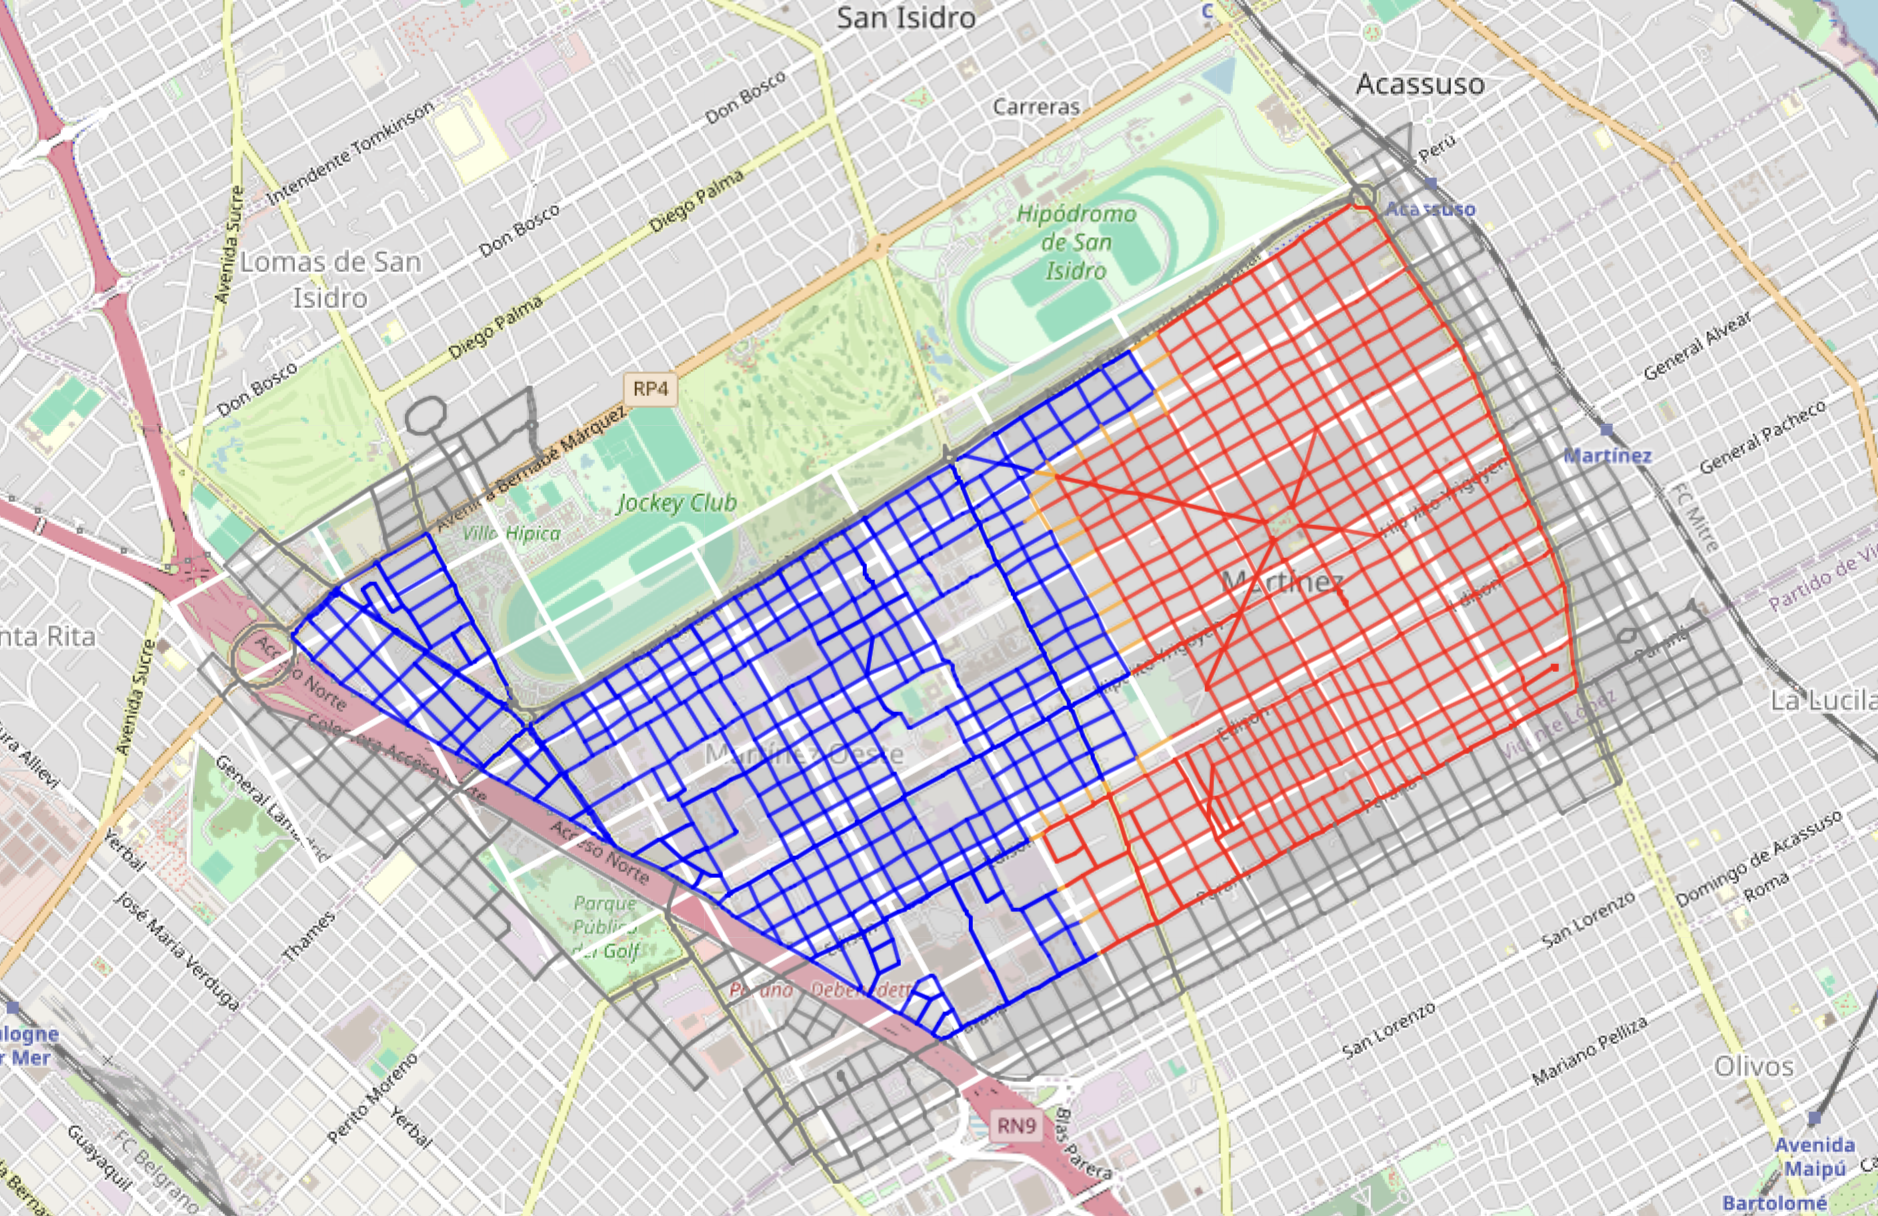
\includegraphics[scale=0.3]{img/zonas_martinex.png}
    \caption{Zonificación}
    \label{fig:zone}
\end{figure}


Similar al modelo principal, vamos a pensar a las calles como aristas y las intersecciones como nodos. Primero tenemos que pensar en cual es la función objetivo de este nuevo modelo. Vamos a querer minimizar la distancia máxima entre los nodos de una zona para poder lograr la forma compacta que buscamos. A través de restricciones flujo vamos a lograr que sean zonas conexas y usando otras restricciones auxiliares vamos a asignar cada nodo a una zona.

\newpage

Dado un grafo $G = (V,E)$,  $d:E\rightarrow \mathbb{R}$ como la distancia de un eje, $q:V\rightarrow \mathbb{R}$ como la demanda de un nodo, $U$ como una cota superior sobre la demanda calculada como $\frac{D_T}K$, es decir, la demanda total sobre la cantidad de zonas. $W$ como la capacidad del camión y $K$ como la  cantidad de zonas que debemos definir, vamos a precisar de las siguientes variables:

\begin{align*}
    X_{ui} &= 
    \begin{cases}
        1 & \text{si el nodo } u \text{ representa la zona } i \\
        0 & \text{caso contrario}
    \end{cases} \\
    Z_{ui} &= 
    \begin{cases}
        1 & \text{si el nodo } u \text{ es asignado a la zona } i \\
        0 & \text{caso contrario}
    \end{cases} \\
    Y_{uv} &= 
    \begin{cases}
        1 & \text{si los nodos } u \text{ y } v \text{ son asignados a zonas distintas}\\
        0 & \text{caso contrario}
    \end{cases} \\
    F_{ij} &= \text{Flujo del eje } ij \\
    D_i &= \text{Distancia máxima de la zona } i
\end{align*}

\begin{align}
    \min \quad & \sum^K_{i=1} D_i \\
    \text{sujeto a} \quad & \sum^K_{i=1} X_{ui} = 1 & \\
    & X_{ui} - X_{vi} \leq Y_{uv} & \forall i = 1\dots k \text{ } \forall (u,v) \in E\\
    & X_{vi} - X_{ui} \leq Y_{uv} & \forall i = 1\dots k \text{ } \forall (u,v) \in E\\
    & X_{ui} + X_{vi} + Y_{uv} \leq 2 & \forall i = 1\dots k \text{ } \forall (u,v) \in E\\
    & \sum_{u\in V} Z_{ui} = 1 & \forall i=1\dots k \\
    & Z_{ui} \leq X_{ui} & \forall i=1\dots k \text{ } \forall u \in V\\
    & F_{uv} + F_{vu} \leq M(1 - Y_{uv}) & \forall (u,v) \in E \\
    & \sum_{v \in \delta^-(u)} F_{uv} - \sum_{v \in \delta^+(u)} F_{uv} \geq 1 - M\sum^K_{i=1}Z_{ui} &\forall u \in V \\
    & D_i \geq d_{uv} (X_{ui} + X_{vi} - 1) & \forall i = 1\dots k \\
    & \sum_{u\in V} X_{ui} q_u \geq 0.9 W & \forall i = 1\dots k \\
    & \sum_{u\in V} X_{ui} q_u \leq 1.05 U & \forall i = 1\dots k \\
    & \sum^K_{i = 1} D_i \geq \frac{K}{1.05} D_i & \forall i = 1\dots k \\
    & \sum^K_{i = 1} D_i \leq \frac{K}{0.95} D_i & \forall i = 1\dots k
\end{align}

En la restricción $(14)$ forzamos a que un nodo se encuentre únicamente en una zona. En las restricciones $(15)$, $(16)$ y $(17)$ relacionamos las variables $X$ e $Y$ de forma de establecer una restricción de asignación de zona a cada para de nodos. Luego en la $(18)$ elegimos un único representante por zona y en la $(19)$ nos aseguramos de que ese representante efectivamente esté asignado a la zona que representa. En $(20)$ y $(21)$ establecemos el flujo que debe haber entre nodos. En la $(22)$ asignamos la distancia máxima de cada zona. En la $(23)$ y $(24)$ restringimos a la zona contra la capacidad del camión para que sea posible recorrerla recolectando en un único viaje. Además, junto a $(25)$ y $(26)$ hacemos que las $K$ zonas sean balanceadas en demanda y distancia.